\chapter{数学导论 - 微积分基础:导数}

\begin{figure}[ht]
  \centering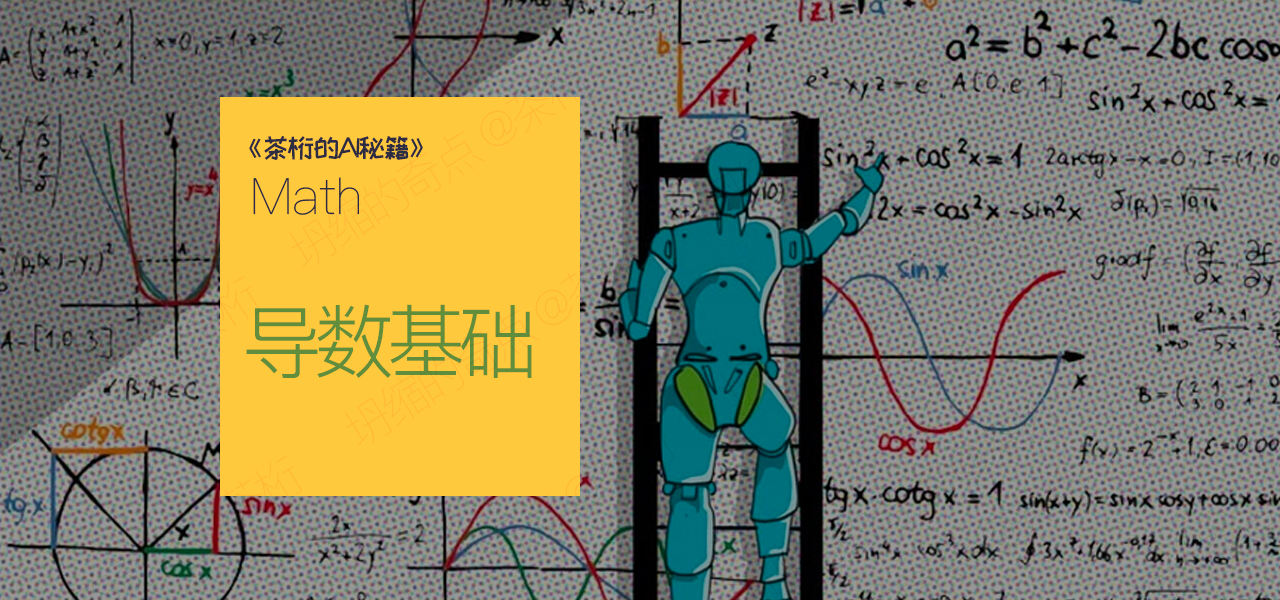
\includegraphics[width=1\textwidth]{asset/茶桁的AI秘籍_Math_2.png}
\end{figure}

\newpage

我们需要用几节课来对一些基础的数学内容进行一下回顾, 能回忆的起来的小伙伴非常优秀, 回忆不起来也没关系, 跟着我的节奏往后走就可以了. 

本节课, 我们先来回顾一下微积分的基础(导数). 

\section{函数}

首先, 我带大家回顾一下: \textbf{函数它是一个什么样的东西}. 

按照我们记忆或者说印象当中的, 函数是左边一个因变量y(通常用y来表示), 右边是一个函数式子: $y=x+1$, 函数式里面包含了次变量. 

我们来看四张图:

\begin{figure}[ht]
  \centering
  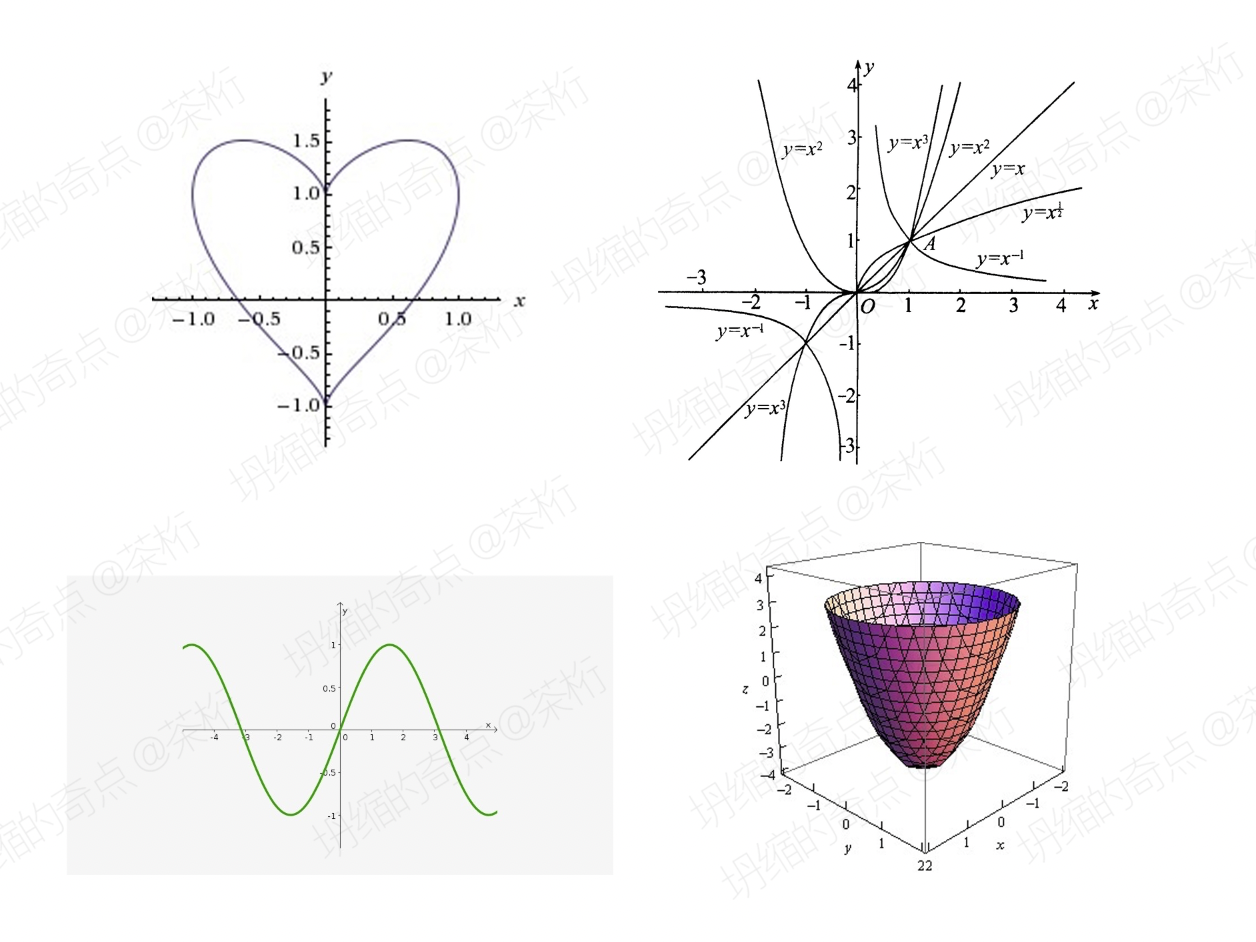
\includegraphics[width=1\textwidth]{asset/fa27e701-ba74-4406-bcb2-7956f4188918.png}
  \caption{多种函数的图形}
  \label{fig:img3_1}
\end{figure}

这些图像, 有的是函数, 有的不是函数. 大家知道这四个图像里面, 哪一个不代表着函数图像吗?

就是左上这个并不是函数. 因为什么呢? 因为它的一个x值对应着两个y值. 就比如说 $x=0$ 这个值, 在上方和下方各对应着两个y的值 $(1.0, -1.0)$. 这是不符合函数定义的. 那其他这几个呢, 都是函数的图像. 如果大家答对了, 我也就安心了, 说明大家对这部分还没有忘. 

函数的形式有很多种: 一次的、二次的、正旋、指数、对数、多元函数等等. 

\begin{align*}
    & y=x^2 & y=sinx \\
    & y=e^x & y={log_2}x \\
    & z=x^2+y^2 & ...
\end{align*}

如果我们抽象一点来看, 可以把函数理解成什么呢?就是我给它一个输入, 然后按照这个函数设定好的规则给我一个输出, 如图 \ref{fig:img3_2}. 

\begin{figure}[ht]
  \centering
  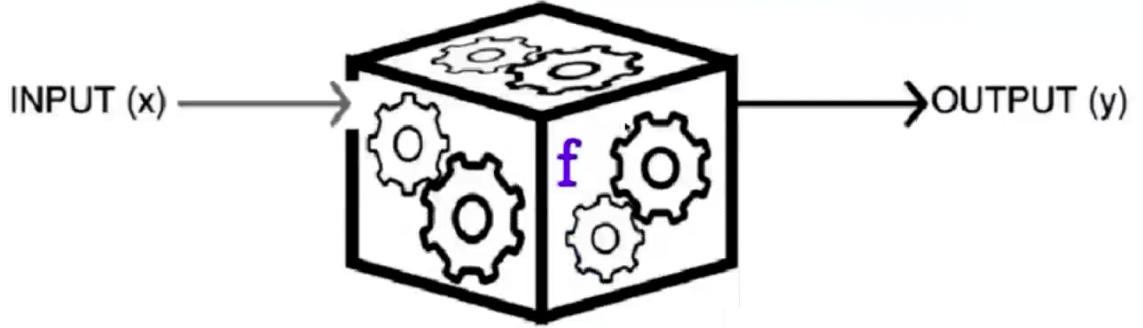
\includegraphics[width=0.5\textwidth]{asset/9f20645c-ef49-4ffd-9178-d01b67c74249.png}
  \caption{什么是函数}
  \label{fig:img3_2}
\end{figure}

拓展讲一下, 大家知道「函数」这个中文是怎么来的吗?\textbf{李善兰}是清代的一个数学家, 他那个时候看到 function 这个词就觉得不能音译过来, 不能跟日本人一样什么词都音译过来, 就是要取一个中文名. 函数就像一个黑盒子一样, 你不需要了解它内部的构造是什么, 你给它一个输入, 它就能按照规定的规则给你一个输出. 所以「函」代表着什么意思?代表的就是盒子包装起来. 比如「石函、剑函」, 基本字义就是「匣, 盒子」的意思. 

除此之外, 李善兰所创立的二次平方根的幂级数展开式, 研究的各种三角函数, 反三角函数和对数函数的幂级数展开式也成为了“十九世纪中国数学界最大成就”. 

李善兰把 function 这个词翻译成了函数,就表示这个规则是装在一个黑盒子里面一样. 更抽象一点, 自变量的数量是可以有很多种. 就是说函数的输入不一定非得是一个, 它有n多个. 你有1,000万个、100万个都行. 但是它输出只有一个. 

\begin{align*}
    x,y,...(\mbox{自变量}) \Rightarrow f(\mbox{函数}) => z(\mbox{因变量})
\end{align*}

这个就叫做多元函数, 就是它的自变量如果超过一个叫做多元函数. 自变量只有一个叫做一元函数. 

\section{导数}

在简单回顾了函数之后, 我们来说一下导数. 

导数这个东西我们怎么样去理解呢?我们用一个运动学的例子带大家理解一下. 

首先我们来看一下图 \ref{fig:img3_3}, 这个坐标系可以看懂吧?这个平面直角坐标系中x轴代表这个自变量, 纵轴代表了因变量. 这个运动问题里面横轴(x轴)就代表了时间, y轴代表了位移. 运动问题:(y: 位移,  x: 时间).

\begin{figure}[ht]
  \centering
  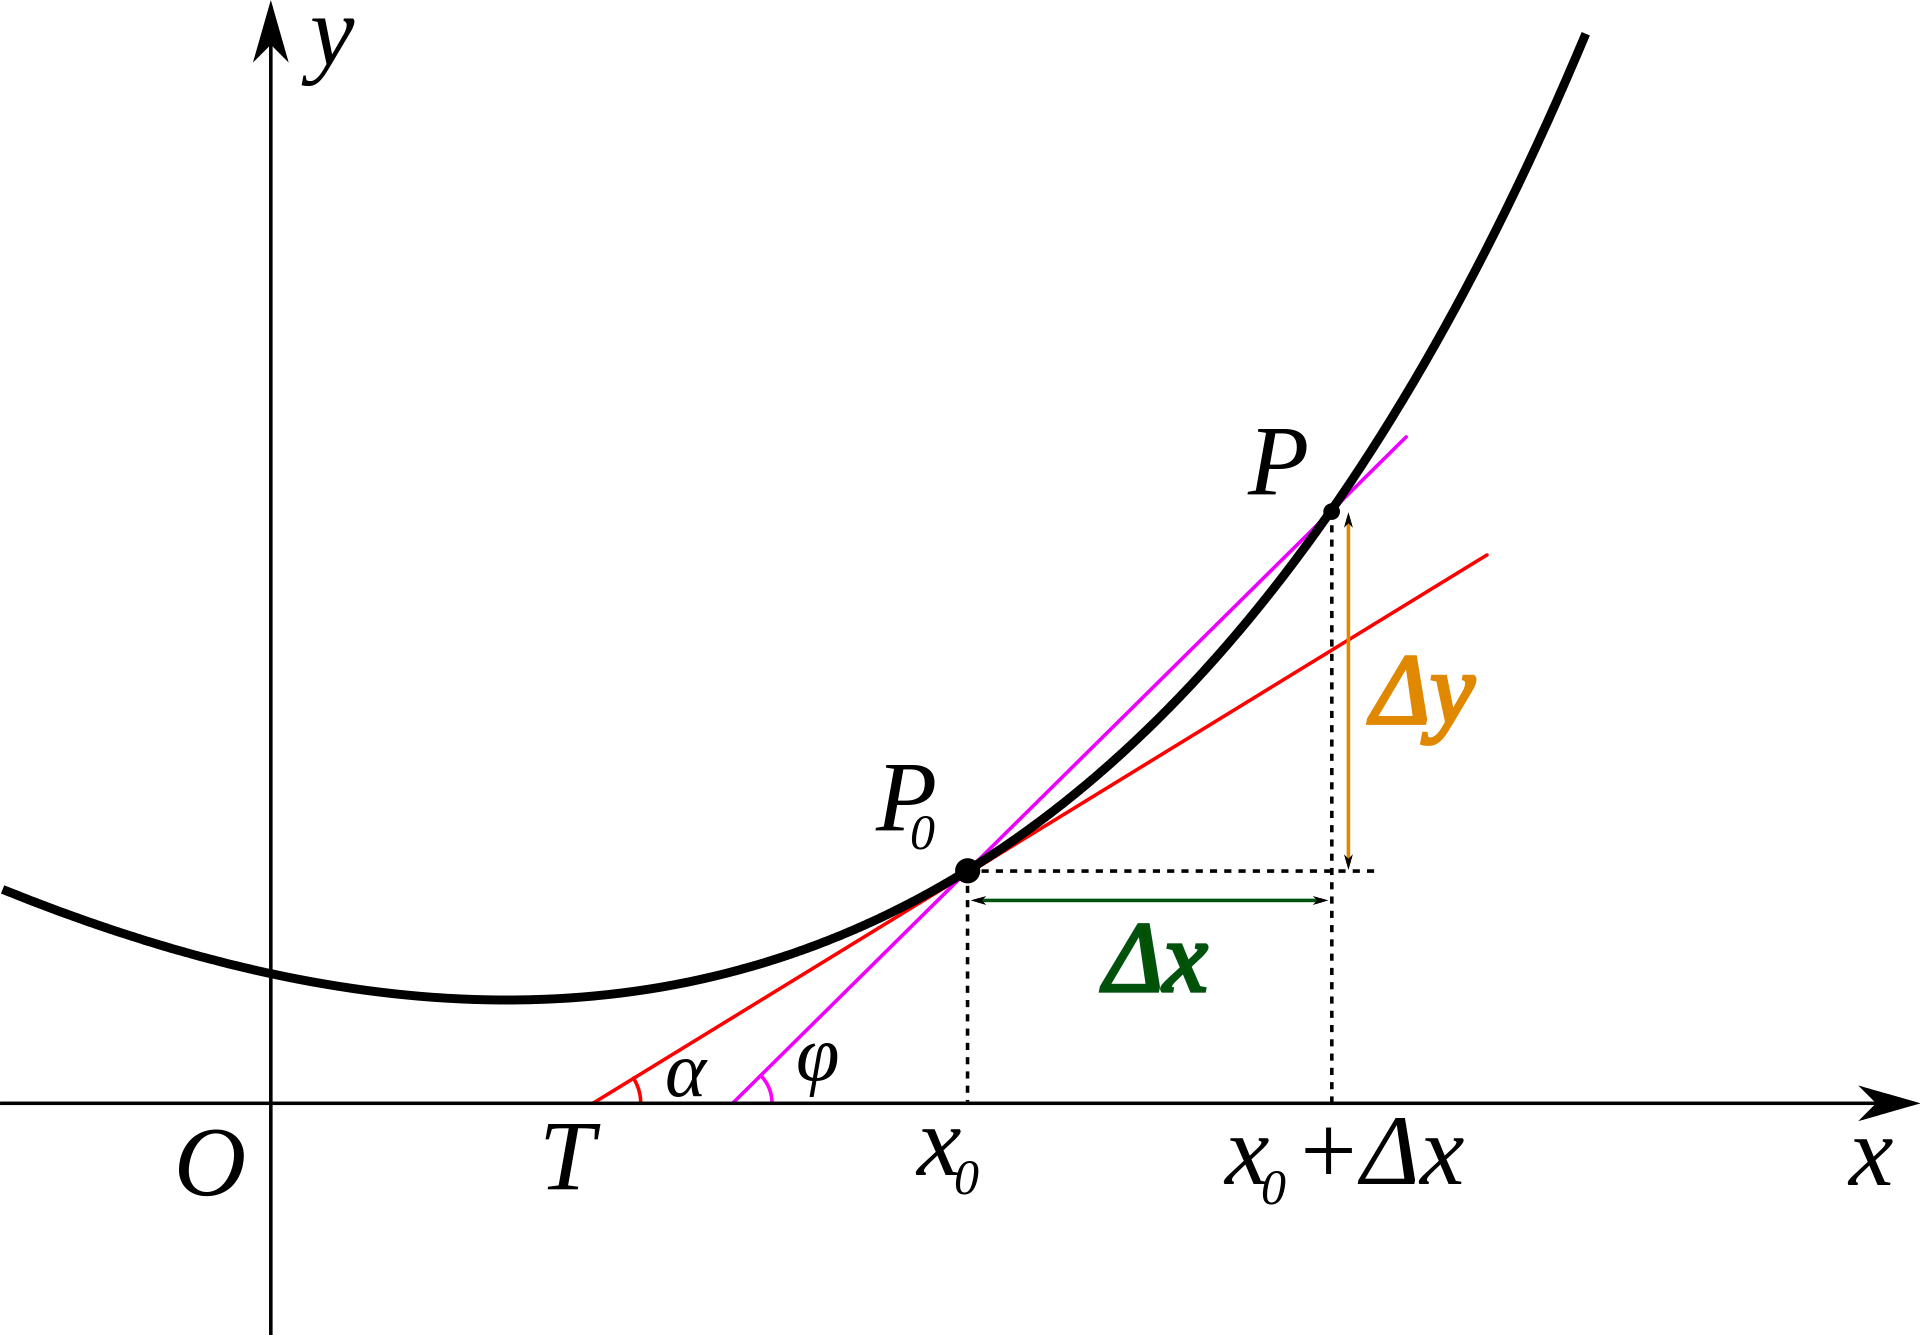
\includegraphics[width=0.7\textwidth]{asset/8b53b1a6-4a67-4402-b86a-b29dab8c535b.png}
  \caption{}
  \label{fig:img3_3}
\end{figure}


我们来看一下这个运动图像是这条黑线, 然后我们来考虑一下$P_0$和$P$这两点. 

如果我们只看这一段, 也就是质点从$P_0$运动到$P$这个位置, 那么它就位移了$\Delta y$, 一共花了$\Delta x$的时间. 我们就能得到$P_0$和$P$这一段运动的平均速度$\overline{v}=\frac{\Delta y}{\Delta x}$. 

在这个过程中, 我们不断的让$P$接近$P_0$,我们并不是说让质点移动, 而是在图像上的两点越来越接近的时候, $\Delta y$和$\Delta x$也在逐步的缩小,  逐步缩小到$P$几乎就要和$P_0$重合. 最终重合的时候, 本来$P$和$P_0$是形成了一条割线(紫色的直线), 当两个点融合为一个点的时候他就退化成了一个切线(红色的直线), 这个切线就是$\Delta x$趋向于0. 在$P$无限接近$P_0$的时候, 我们就是在求$P_0$这个瞬时速度. 基于之前的分析, 那么我们就得到瞬时速度公式:

\begin{align*}
  \lim_{\Delta x\to0} \frac{\Delta y}{\Delta x}=\tan a
\end{align*}

我来解释一下这个公式, $\lim$ 表示取极限的意思, $\Delta x \to 0$表示$\Delta x$趋近于0,  整个公式就是$\Delta x$趋近于0的时候$\frac{\Delta y}{\Delta x}$计算结果等于$\tan a$, 也就是正切值. 也就是$\angle \alpha$这个三角形中对边比上临边, 如图 \ref{fig:img3_4}:

\begin{figure}[ht]
  \centering
  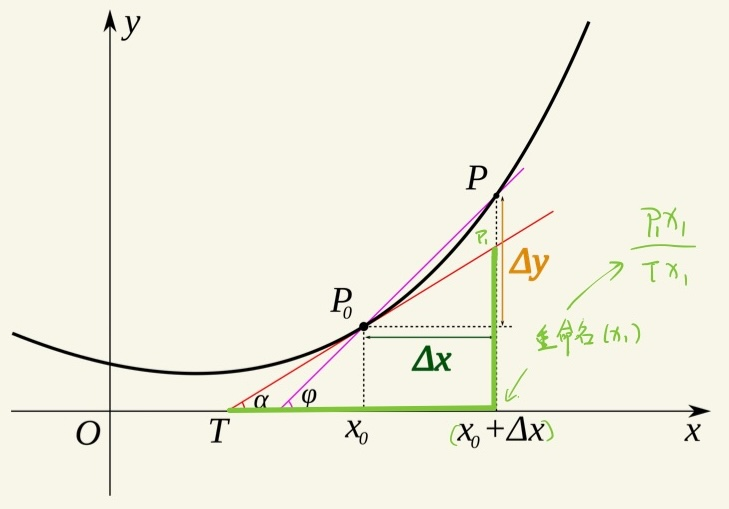
\includegraphics[width=0.8\textwidth]{asset/ac2df882-fb9f-4ddc-ae48-888ff4dec6a6.jpg}
  \caption{}
  \label{fig:img3_4}
\end{figure}

其实并不是说是我们如图看到的那两条线段就是$\Delta y$和$\Delta x$, 而是说他们代表的比例是相等的, 因为它们已经退化成了切线了, 所以我们只能用这个角度来表示. 

\section{导数与微分(一元函数)}

现在我们就可以引入导数正式的定义:

\begin{align*}
  y'=f'(x)=\lim_{h \to 0}\frac{f(x+h)-f(x)}{(x+h)-x}
\end{align*}

大家不用看到这个数学公式就非常紧张, 没必要. 从我学习的经验来看, 其实很多大白话能说清楚的事情, 非要起一个学术的名字, 非要用一个听不懂的概念来说. 其实当我们真正不被字符和符号来迷惑的时候, 就会觉得这些东西非常简单. 

那这个导数是什么意思呢?一般导数我们都会用 $'$ 来表示, 比如公式中的$y'$, $f'$, 它是相应函数的导数. 比如$f'(x)$就是表示$f(x)$的导数. 它的定义其实就是我们的趋近过程, 我们取两个点, 一个是$x+h$,  一个是$x$, 也就是图像中的 $x_0+\Delta x$ 和 $x_0$ 这两个点, 当$h$无限趋近于0, 分子部分是函数$f(x+h)$ 和函数$f(x)$的差值(也就是图像中的$\Delta y$), 分母部分是$(x+h)-x$,就相当于图像中横坐标的差值, 也就是$\Delta x$. 那我们的导数的定义就出来了, 就是我们求图像的某一段, 其纵坐标的差比横坐标的差, 当两点距离越来越小的时候, 我们就得到其导数了. 也就是在图像中, 我们得到了$P_0$这个点上的切线的斜率. 

接着就是一些相关定义:

\begin{itemize}
  \item $y$被称作$y'$的原函数
  \item $y'$被称作$y$的导函数(导数)
  \item 微分:当自变量x的变化趋于无穷小时($dx$), 因变量f(x)的变化情况($df(x)$). 
\end{itemize}

\begin{align*}
  df(x)=f'(x)dx
\end{align*}

微分的概念很多人容易和导数混淆, 它们的概念是有点相近, 但是代表的是不同的含义. 比如说在上面那个图像中, 质点从$P_0$点向$P$移动, 这个移动量几乎不可察觉, y也就是一点点的变化. 不管移动了多少, 也就是相当于横轴上$x_0$向右移动一点点, 那这个图像也就向上移动了一点. 当自变量x增加或者减少了一点的时候, 因变量$f(x)$增加或者减少了多少. 这个自变量和因变量的变化量, 都用$d+\mbox{变量}$来表示. 这个$d$就是表示微分的意思. 那么$dx$就是x具体变化了多少量(当然这个量是非常小的, 可以想作趋向于0), 与之对应的, $df(x)$也就是因变量$f(x)$具体变化了多少量. 

在神经网络中, 优化反向传播, 也就是反向传递这个导数的过程. 所以说, 导数还是一个很核心的一个概念. 

下面这个就是我们常见的一些函数的导数, 这些函数也就是一些初等基本函数. 

\begin{align*}
  & C'=0 & (x^n)'=nx^{n-1} \\
  & (sinx)'=cosx & (cosx)'=-sinx \\
  & (a^x)'=a^x \ln a & (e^x)'=e^x \\
  & (log_a{x})'=\frac{1}{x}log_a{e} & (\ln x)'=\frac{1}{x}
\end{align*}

来看一个求导的例子, 我们利用导数的定义求证一下其中一个函数导数: $(sinx)'=cosx$

\begin{align*}
  \mbox{求证}:&  (sinx)'=cosx \\
  \mbox{证明}:& \mbox{令}f(x)=sinx \\
  \mbox{因为}:& f'(x)=(sinx)' \\ 
  & =\lim_{h\to0}\frac{f(x+h)-f(x)}{(x+h)-x} \\
  & =\lim_{h\to0}\frac{sin(x+h) - sinx}{h} \\ 
  & =\lim_{h\to0}\frac{sinx cosh + cosx sinh - sinx}{h} \\
  & =\lim_{h\to0}(\frac{sinx - sinx}{h} + \frac{cosx sinh}{h}) \\
  \mbox{因为}: & \lim_{h\to 0}cosh=1, \lim_{h\to0}\frac{sinh}{h}=1 \\
  \mbox{所以}: & \mbox{原式} =cosx
\end{align*}

中间转化的过程中用到了三角函数的「和差化积」, 有兴趣的可以自己 \href{https://www.google.com/search?q=%E5%92%8C%E5%B7%AE%E5%8C%96%E7%A7%AF&sourceid=chrome&ie=UTF-8}{Google一下看看}. 

这个推理过程我稍微解释一下, 当h取值无限小的时候, 那么$cosh=1$,  而当h取值无限小的时候, $sinh=h$. 所以有了这一步, 其他的部分就相对容易看懂了. 

我们再说一下导数的运算法则, 如果有两个函数, 那它们组合在一起的这个导数是什么样的形式呢?其实也就四种情况:\textbf{相加减、和常数相乘、两个函数相乘、两个函数相除}, 结果如下: 

导数的运算法则: 设 $u=u(x), v=v(x)$ 可导, 则:

\begin{align*}
  & (1) (u\pm v)'=u'\pm v'; &(2) (cu)'=cu' (C\mbox{是常数}); \\
  & (3) (uv)'=u'v+uv'; &(4) (\frac{u}{v})'=\frac{u'v-uv'}{v^2}(v \ne 0)
\end{align*}

这里就不带大家一一去看了, 主要是靠大家自己在课后的时候去琢磨一下, 这个部分也不会特别难. 

再来带大家看一个证明题, 就是我刚才说的导数运算法则里面两个函数乘在一起, 它们的导数为什么是这样的一个形式. u和v乘在一起, 然后对它整体进行求导为什么是一个函数的导数乘上另外一个函数再加上另外一个函数的导数乘上这个函数. 我们来看一下这个证明. 


\begin{align*}
  \mbox{求证:} &  (uv)'=u'v + uv' \\
  \mbox{证明:} & \mbox{令} u = f(x), v = g(x) \\
  & \mbox{则} (uv)' = (f(x)g(x))' \\ 
  & = \lim_{h\to 0}\frac{f(x+h)g(x+h) - f(x)g(x)}{(x+h - x)} \\
  & =\lim_{h\to0}\frac{f(x+h)g(x+h)-f(x+h)g(x)+f(x+h)g(x)-f(x)g(x)}{h} \\
  & =\lim_{h\to0}\frac{f(x+h)(g(x+h)-g(x)) +g(x)(f(x+h)-f(x))}{h} \\
  & =\lim_{h\to0}\left[f(x+h) \cdot \frac{g(x+h)-g(x)}{h} + g(x)\cdot \frac{f(x+h)-f(x)}{h} \right] \\
  & =f(x)g'(x) + g(x)f'(x) \\
  & \Rightarrow u'v + uv'
\end{align*}


同样的, 我们这两个函数, 令它等于 $f(x)$和$g(x)$ 就是为了方便, 其实都一样的. 我们同样是套用这个导数的定义式去做. 导数的定义式不光能让你求出具体一个函数的导数是什么, 还能让你求出两个函数乘在一起的导数. 

导数计算在机器学习中什么场景用的最多? 目标函数或者说损失函数, 不管是图像处理还是自然源处理, 都有个目标函数. 目标函数怎么优化, 就是不断的求导, 然后把这个导数一层一层的向前面的那些神经网络层传, 反向传播过去, 从最后一层传到前面一层. 在这个过程当中导数是非常关键. 

不知道大家有没有听过这么一个词:「\textit{随机梯度下降}」\footnote{随机梯度下降, 也就是SGD. }. 梯度下降其实就是求导, 不断的对神经网络里面的参数进行优化, 也是减去相应的导数值乘上学习率. 不管你是什么样的优化方法, 即便不是随机剃度下降, 它都是以求导计算为基础的. 所以有神经网络地方, 都离不开求导. 

\section{偏导数}

导数是针对一元函数的, 自变量只有一个. 但是我们在自然界当中经常会遇到多元函数的形式, 一个自变量不能按照既定的规则给出输出, 需要很多个输入. 

比如说$x_1, x_2$, 一直到$x_n$. 这个函数的映射法则之下才能给到我们一个输出, 这个叫做多元函数. 多元函数有一个问题, 那就是既然自变量这么多, 函数y相对于每一个自变量不都有一个导数吗?所以因变量相对于每一个自变量都有一个导数, 这每一个导数呢都叫做偏导数. 

多元函数:$y=f(x_1, x_2, ..., x_n)$

\begin{itemize}
  \item 因变量相对于每一个自变量均有一个导数, 称为偏导数
  \item 形式:$\frac{\partial y}{\partial x_1}, \frac{\partial y}{\partial x_2}, ..., \frac{\partial y}{\partial x_n}$
  \item 如何求:求解某一自变量的偏导数时, 将其它自变量视作常数
  \item 梯度:各个方向的偏导数构成的向量, ($\frac{\partial y}{\partial x_1},\frac{\partial y}{\partial x_2}, ..., \frac{\partial y}{\partial x_n}$)
  \item 梯度的表记:$\nabla f(x_1, x_2, ..., x_n)$或者$grad f(x_1, x_2, ..., x_n)$
\end{itemize}

大家看到多元函数觉得好复杂, 自变量相互之间还有影响, 其实它们压根就没有影响. 求解的时候全部把它看作是常数, 就不用理它. 

梯度就是各个方向或者说各个字面上偏导数构成的一个向量. 向量是什么意思大家明白吗?向量和标量是相对的, 标量是只有数值没有方向. 比如说我有2个苹果、我有3个梨、我有4个橘子. 它就表示数量关系, 没有方向. 向量是有数值大小有方向, 在给定空间内 相对于任意一点在各个分量方向上的变化量的统一表述而已. 比如向量$(1, 1, 1)$ 就代表相对于三维空间中的任意一点在三个坐标轴方向上变化了 $(1 \quad 1 \quad 1)$. 

比如说在物理学里面速度的定义是很严谨的, 我们日常生活中说的速度只是一个数值没有带方向, 但是在物理学里面速度就是一个向量, 它不光有数值还有方向. 在物理学里面速度不光说他是70公里每小时, 还得说他速度朝哪个方向. 

我们来看一个例子: 求多元函数$y=f(x_1, x_2)=x_1^2 + x_1x_2 + sinx_2$的偏导数:

\begin{align*}
  \mbox{解}: & \frac{\partial y}{\partial x_1}=2x_1+x_2 \\
& \frac{\partial y}{\partial x_2}=x_1+cossx_2 \\
\end{align*}

我们之前讲过, 求某一个自变量的偏导数的时候, 把另外一个量视作常数. 

这个函数对于这个$x_1$这个自变量的偏导数是什么呢?$x_1$的平方, 按之前讲的求导法则, 它是两倍的$x_1$对吧?$(x^n)'=nx^{n-1}$, 如果不熟悉的同学再回去看一下常用基本初等函数的导数是什么. 那个里面的函数, 会经常用所以大家多看一下. 

然后再来看第二项$x_1x_2$, 在这里把$x_2$当做常数, 所以它就相当于一个$Cx_1$, $Cx_1$求导, 留下的就是$C$, 就是$x_2$. 最后一项$sinx_2$里面没有$x_1$, 所以这一项它就相当于是常数$C$, 常数求导它就是0. 为什么常数求导是0呢, 因为如果你这个函数它是一个常函数, 它在这个直角坐标器里面不管x取值是多少, y值都是一样的, 就是一条横线. 

比如说$f(x)$等于3,不管你这个x等于几,这个函数值都是3, 它就是一条水平的直线. 水平直线的变化率就是0, 导数也表示一个变化率. 

然后再看一下第二个y关于$x_2$的导数, 我们用同样的方法. 首先第一项里面不含$x_2$所以pass, 它求导就是0. 第二项里面它是$x_1$乘上$x_2$, 在这里$x_1$相当于常数, 所以$x_1$乘$x_2$求导就得到$x_1$. 最后一项$sinx_2$求导就是$cosx_2$, 这个我们之前有证明. 

关于微积分的部分我们在这节导数导论课里面就告一段落了. 但是导论课并没有结束, 后面还有线性代数基础(矩阵)、概率 \& 统计基础(随机变量)、图论(图的概念), 我们放在下一节课中再讲. 